\section{Forward neutron detector system}
\subsection{Neutron Counter}

\begin{figure}[htbp]
  \centering
  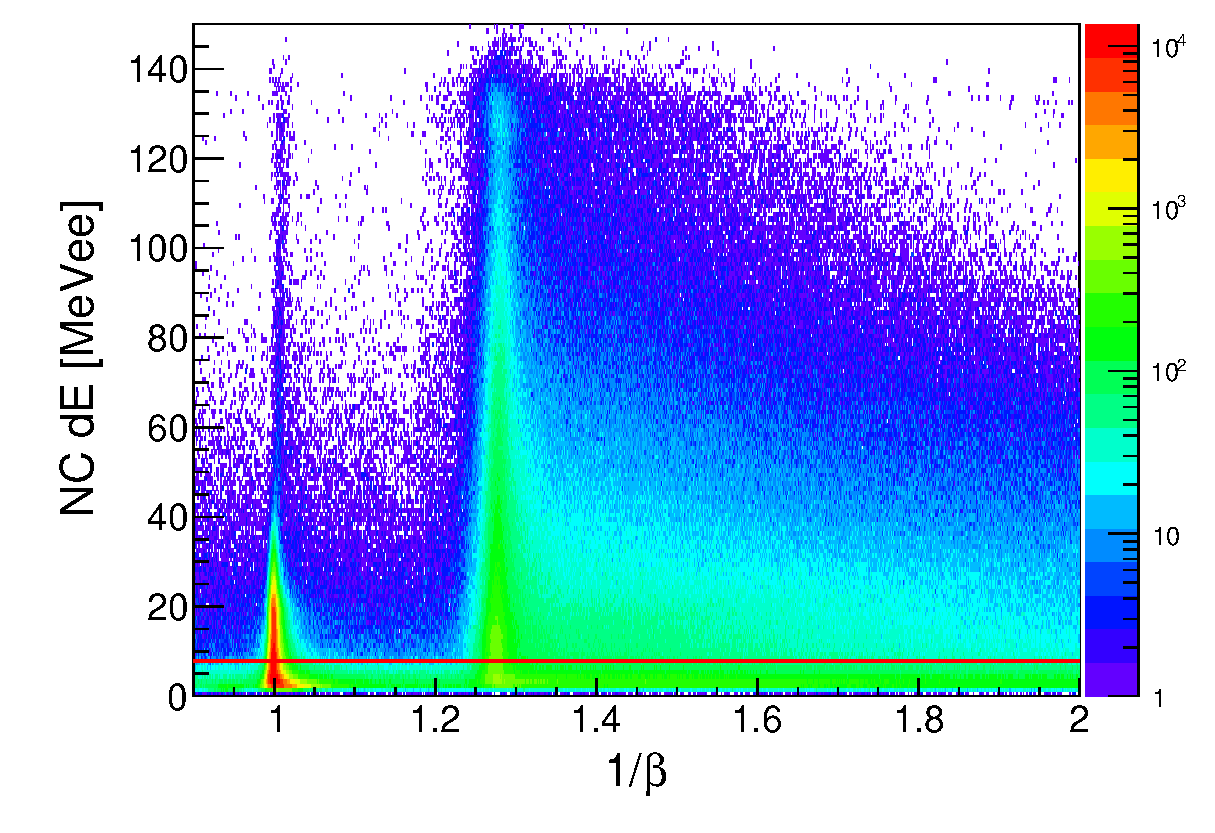
\includegraphics[width=8cm]{../pic/Run78/NC/NC_overbeta_dE.eps}
  \caption{
    This figure shows a scattered plot of $1/\beta$ and energy deposit.
    $\gamma$-ray events was observed at $1/\beta=1$.
    The locus at $\beta=1.3$ corresponds to quasi-elastic scattering events.
  }
  \label{fig:NC_beta}
\end{figure}

\begin{figure}[htbp]
  \centering
  \begin{tabular}{cc}
    \begin{minipage}{0.5\hsize}
      \includegraphics[width=5cm]{../pic/Run78/NC/NC_overbeta_noise.eps}
    \end{minipage}

    \begin{minipage}{0.5\hsize}
      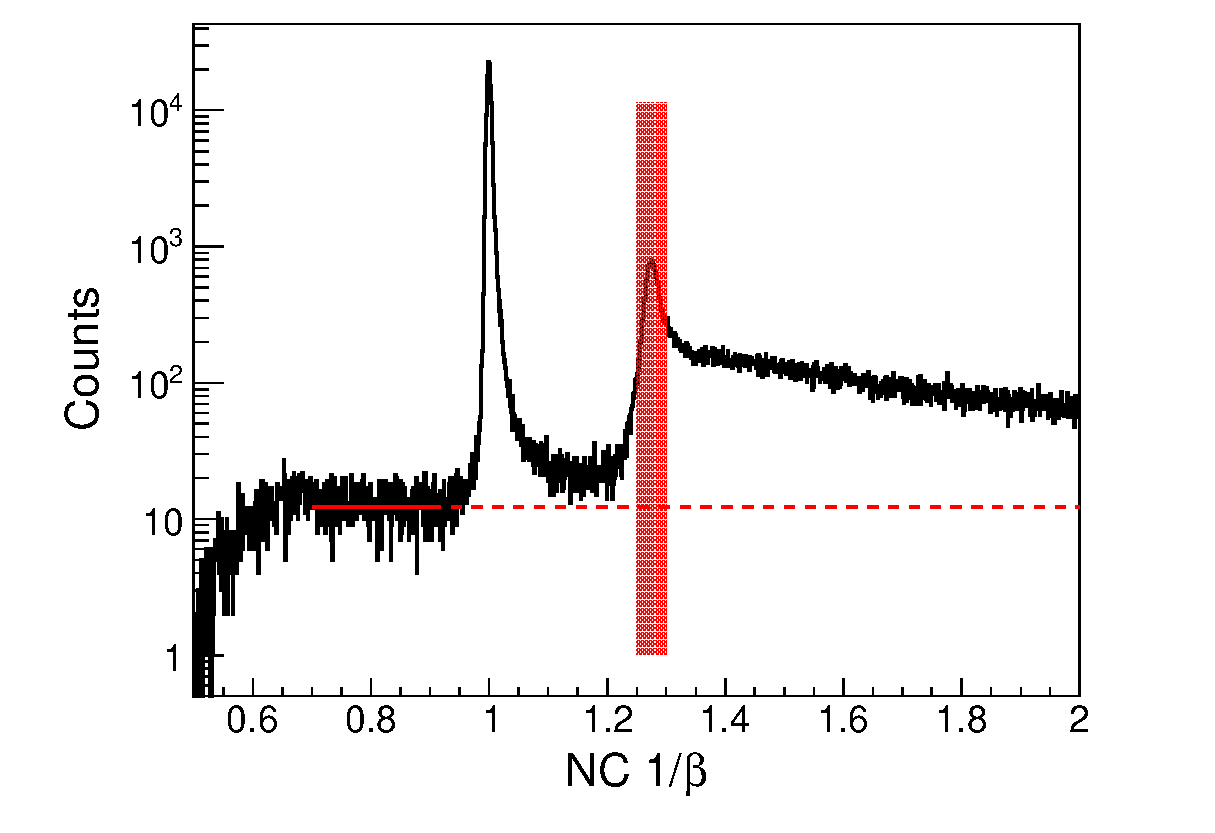
\includegraphics[width=5cm]{../pic/Run78/NC/NC_overbeta_select.eps}
    \end{minipage}
  \end{tabular}
  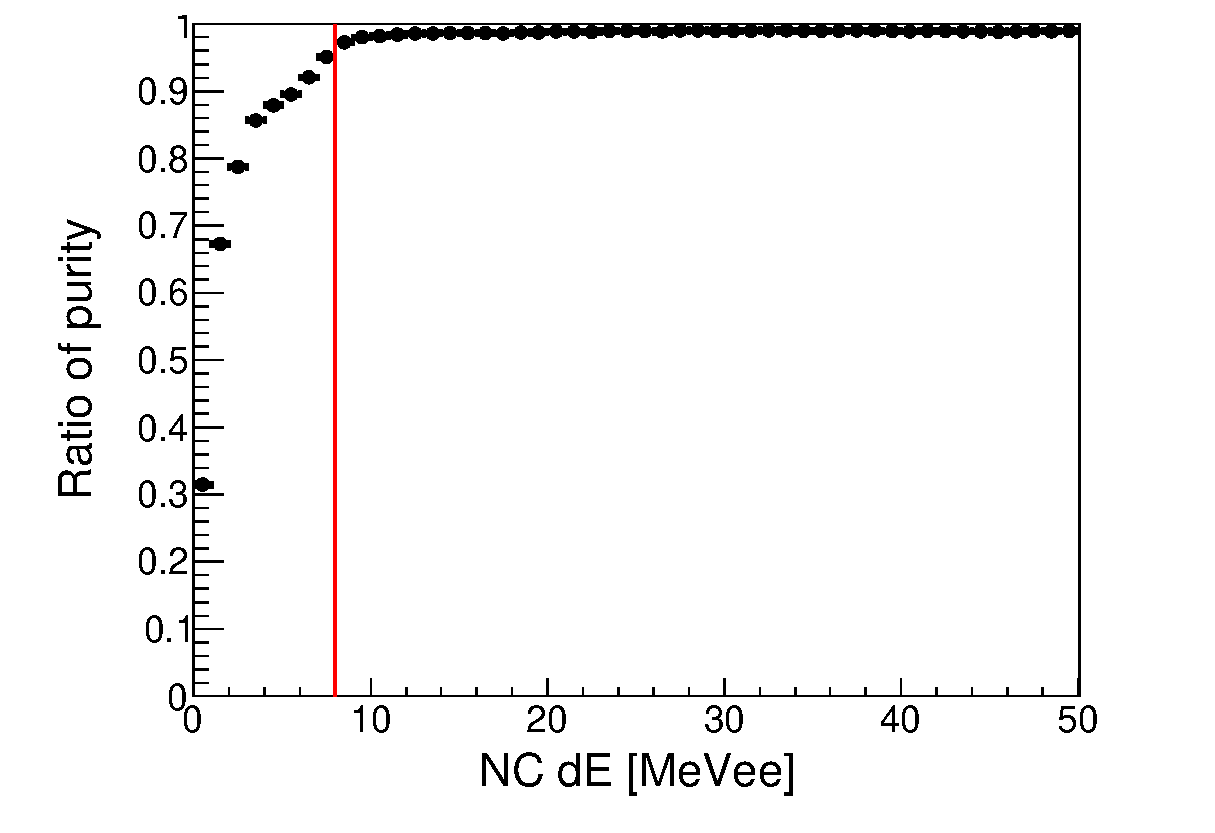
\includegraphics[width=8cm]{../pic/Run78/NC/NC_purity.eps}
  \caption{
    Up figures show $1/\beta$ distribution with a specific dE range.
    Left figure and rigght figure show about $dE=2\sim3 MeVee$ and $dE=8\sim9 MeVee$, respectively.
    The Red line indicates the background level which estimated at $1/\beta=0.7\sim0.9$.
    The Red hatch region indicates a integral range as a signal.\newline
    The down figure shows the $dE$ dependency of the ratio of signal and background.
    The Red line indicates 8$MeVee$ as the online threshold level.
  }
  \label{fig:NC_purity}
\end{figure}

Neutral particles scattered forward direction was not bent by the Ushiwaka magnet and was detected by the NC.
The BVC	rejected the charged particle just upstream of the Ushiwaka, whose purpose was mainly caused by the beam.
Also, the CVC rejected the charged particle just upstream of the NC, whose purpose was the guarantee that the particle was neutral just before the NC.
The flight-length was calculated from the reaction vertex point and the hit position of the NC.
The hit position of the x-axis was determined from the counter placed position. 
The hit position of the vertical axis was calculated from the effective light velocity of the NC and timing signal difference of the up and the bottom PMT.
The effective light velocity was evaluated using a $^{90}Sr$ source measurement changing the position.
The hit position of the z-axis was used as the center of the counter because the reaction point was unknown due to the neutral charge.
The time-of-flight was evaluated from the timing of the T0 and the NC to subtract the time-of-flight of the kaon beam.
The velocity of the forward neutral particle was calculated from the flight length and the time-of-flight.

Fig\ref{fig:NC_beta} shows the scatter plot of the $1/\beta$ and energy deposit.
The NC was set the threshold of a signal at $1/10$ of MIP.
A low energy deposit has many backgrounds, which was estimated in the unphysical region, $1/\beta=0.7\sim0.9$.
And purity of neutron events was estimated using quasi-elastic events ($1/\beta 1.25 \sim 1.30$).
These figures were shown in Fig\ref{fig:NC_purity}.
The purity of the NC was saturated at 8MeVee, so we adopted this value as the offline threshold.\\

The calibration of the NC was first performed using the $\pi^-$ beam through run.
In this calibration, the ADC was calibrated to the energy deposit using the MIP of $1GeV/c$ $\pi^-$.
The time offset was roughly calibrated using the $1GeV/c$ $\pi^-$ beam.
These calibration runs were performed several times in the production period.

More fine tuning for the time offset was performed using a $\gamma$-ray which was located at $\beta=1$ in the production run.
As a result, the resolution of the NC became about 140ps as the sum of all segments through the whole production period, which was shown in Fig\ref{fig:NC_offset}.\\
The stability was checked about time and segment.
The time stability was checked to divide some period in the production period and segment stability was checked through the whole production period due to statistics,
which was shown in Fig\ref{fig:NC_stable}.\\

After the calibration, the missing mass spectra were shown in Fig\ref{fig:KN_MM}, in which spectra tagged decay particles by the CDS also were plotted.

\begin{figure}[htbp]
  \centering
  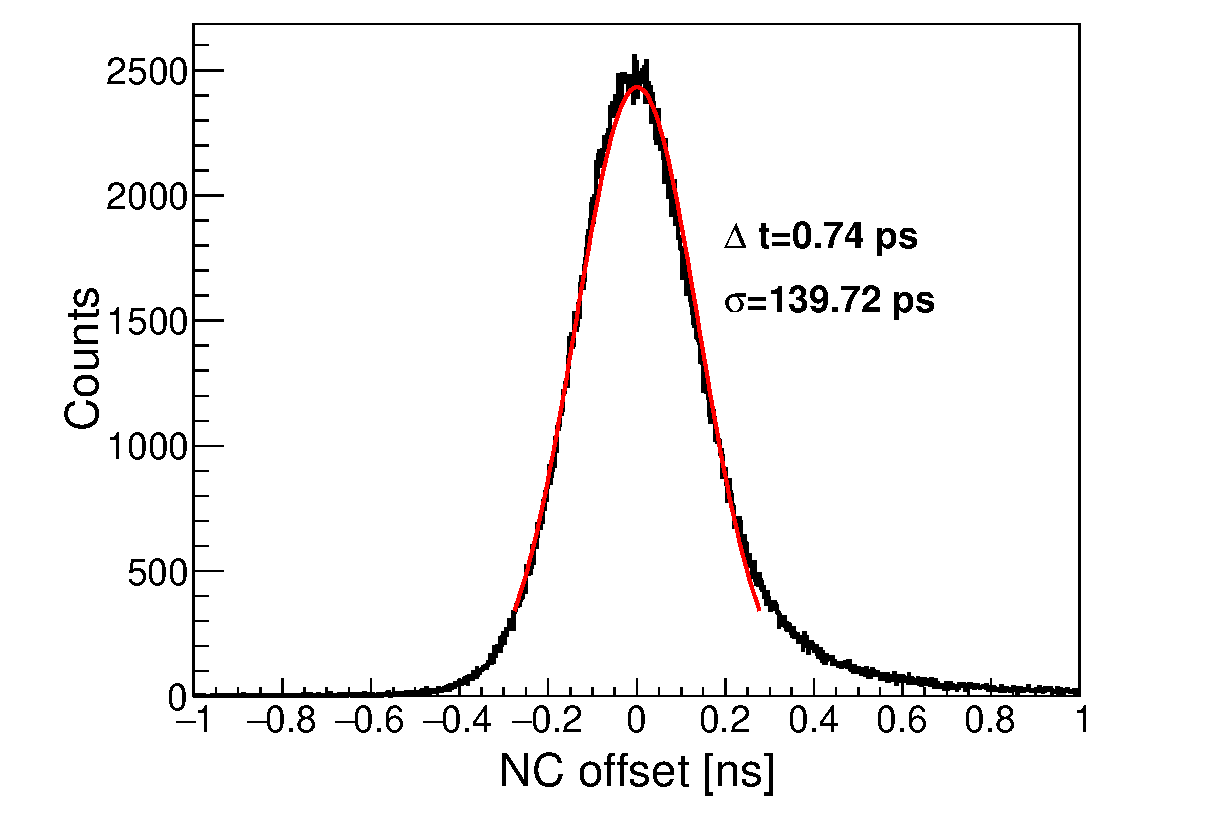
\includegraphics[width=7cm]{../pic/Run78/NC/NC_offset.eps}
  \caption{
    This figure shows the $\gamma$-ray peak in $1/\beta$ distribution with the 8 MeVee offline threshold.
    Fitted gaussian was shown as red slope and mean and $\sigma$ value was indicated at the same figure.
  }
  \label{fig:NC_offset}
\end{figure}

\begin{figure}[htbp]
  \centering
  \begin{tabular}{cc}
    \begin{minipage}{0.5\hsize}
      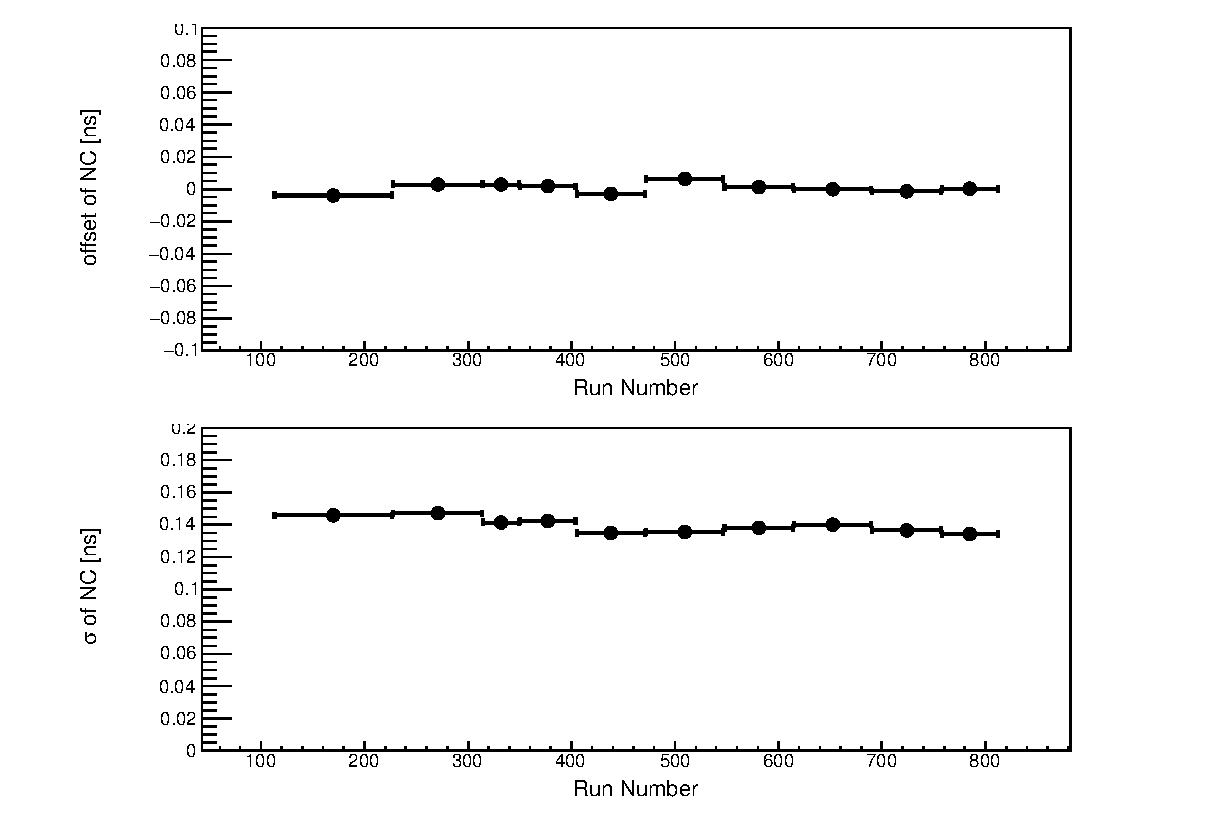
\includegraphics[width=6cm]{../pic/Run78/NC/NC_offset_rundev.eps}
    \end{minipage}
    \begin{minipage}{0.5\hsize}
      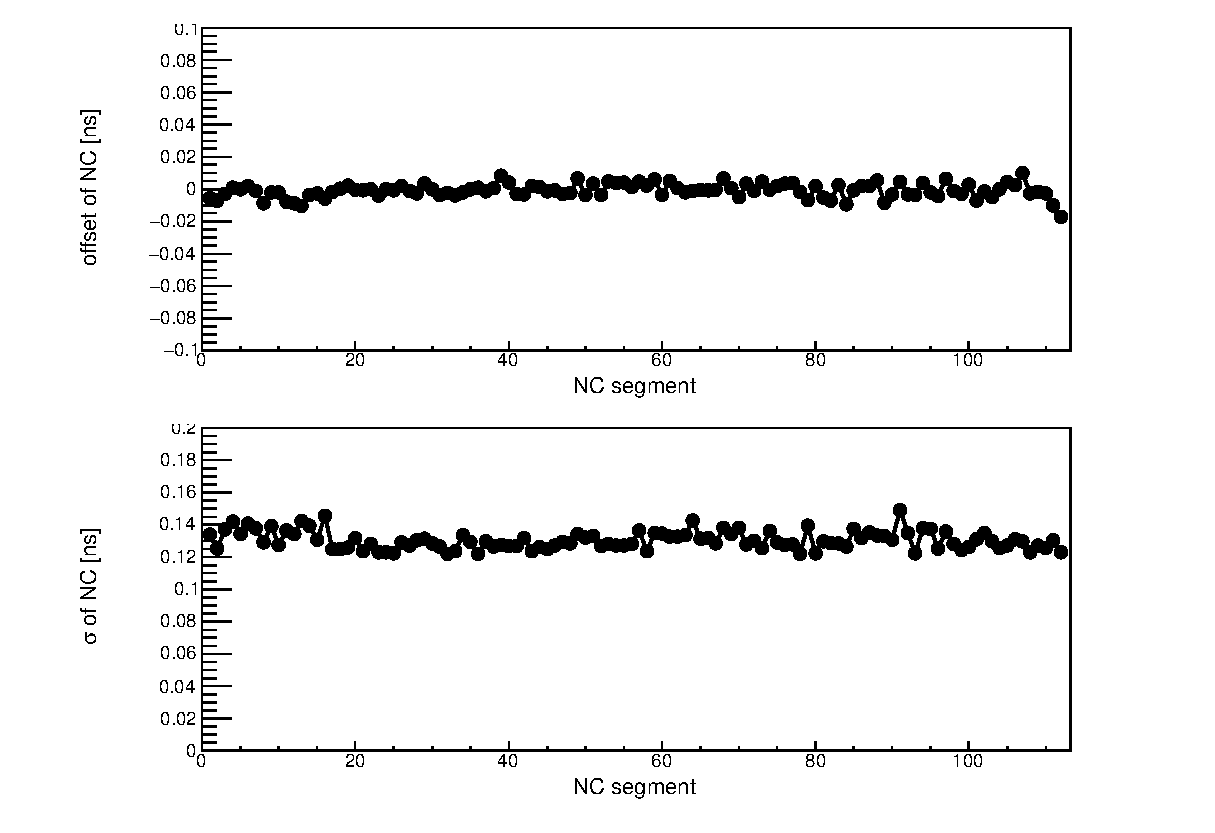
\includegraphics[width=6cm]{../pic/Run78/NC/NC_offset_seg.eps}
    \end{minipage}
  \end{tabular}
  \caption{
    These figures show the stability of the NC performance.
    The above figure indicates the fluctuations of the $\gamma$-ray peak and the down figure indicates the time resolution of the NC.
    The right figure and left figures show run dependency and segment dependency, respectively.
  }
  \label{fig:NC_stable}
\end{figure}

Fig\ref{fig:NC_stable} was shows stability of the NC dureing production run and segment dependency.\\

\begin{figure}[htbp]
  \centering
  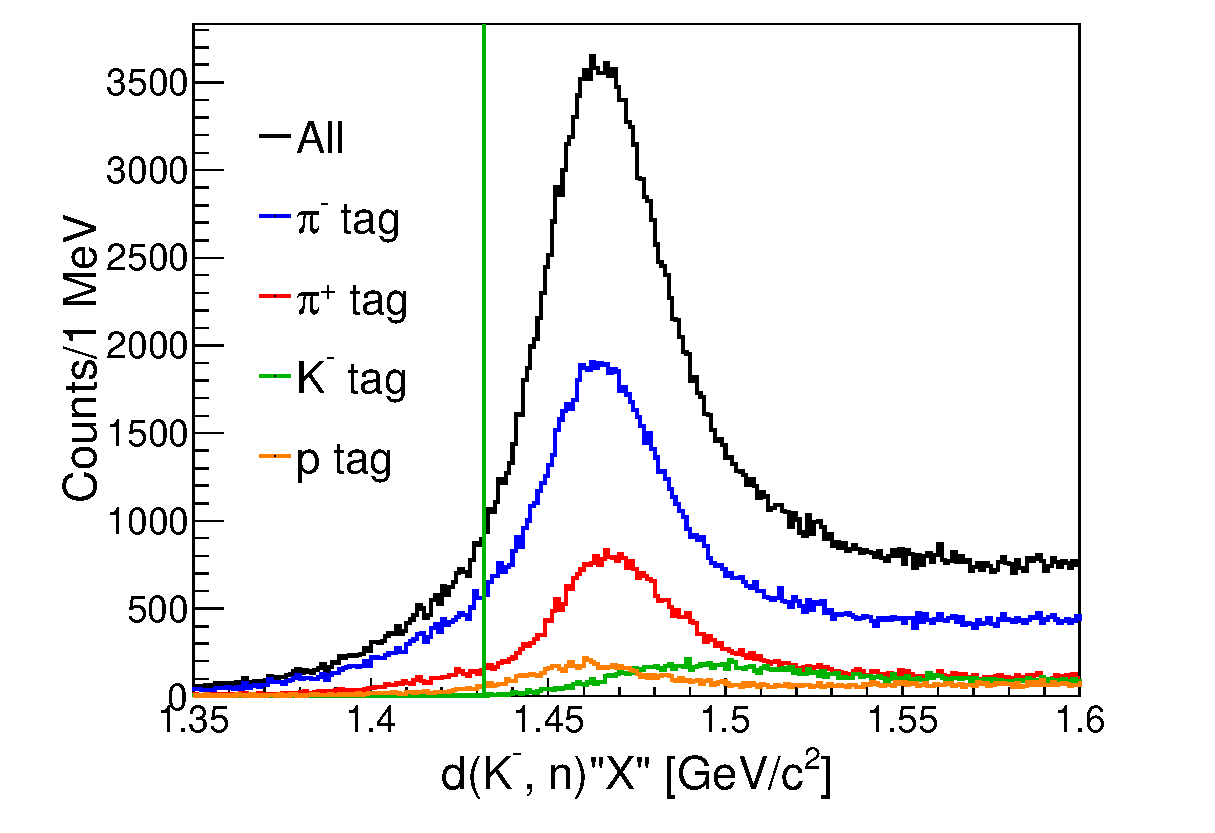
\includegraphics[width=10cm]{../pic/Dron/KN_ana/KN_MM.eps}
  \caption{
    This figure shows $d(K^-, n)"X"$ missing mass.
    The black plot indicates all data and color plots indicate data with the CDS particle tag.
  }
  \label{fig:KN_MM}
\end{figure}
